Anomaly detection is the task of identifying samples that deviate significantly from the expected distribution of normal data. In computer vision, this usually means detecting images or regions whose appearance is inconsistent with the visual patterns observed during training. In industrial inspection, anomaly detection is particularly relevant because defective samples are often rare, heterogeneous, and difficult to collect in a representative way.\cite{li_survey_2025}

Depending on the formulation, visual anomaly detection may operate at different levels of granularity. Some methods produce an \textbf{image-level anomaly score}, indicating whether an image is normal or abnormal as a whole, while others also provide a \textbf{pixel-level anomaly map} that localizes suspicious regions. This distinction is important in industrial settings, where both the decision itself and the interpretability of the detected defect can be relevant.\cite{li_survey_2025}

A common scenario in industrial practice is that abundant normal samples are available, whereas anomalous examples are scarce or completely unavailable. For this reason, many modern anomaly detection methods are designed to learn only the distribution of normal data and to treat deviations from that distribution as potential anomalies.\cite{li_survey_2025} This setting is especially attractive when defects are difficult to enumerate in advance or when collecting defective products would be impractical.

From a methodological perspective, deep-learning-based anomaly detection methods can be grouped into several broad families, including reconstruction-based approaches, feature-embedding methods, teacher--student models, memory-bank methods, and hybrid approaches.\cite{li_survey_2025} Although these methods differ in architecture and supervision signals, they share the same central objective: building a representation of normality that makes abnormal patterns stand out at inference time.

\begin{figure}[h]
    \centering
    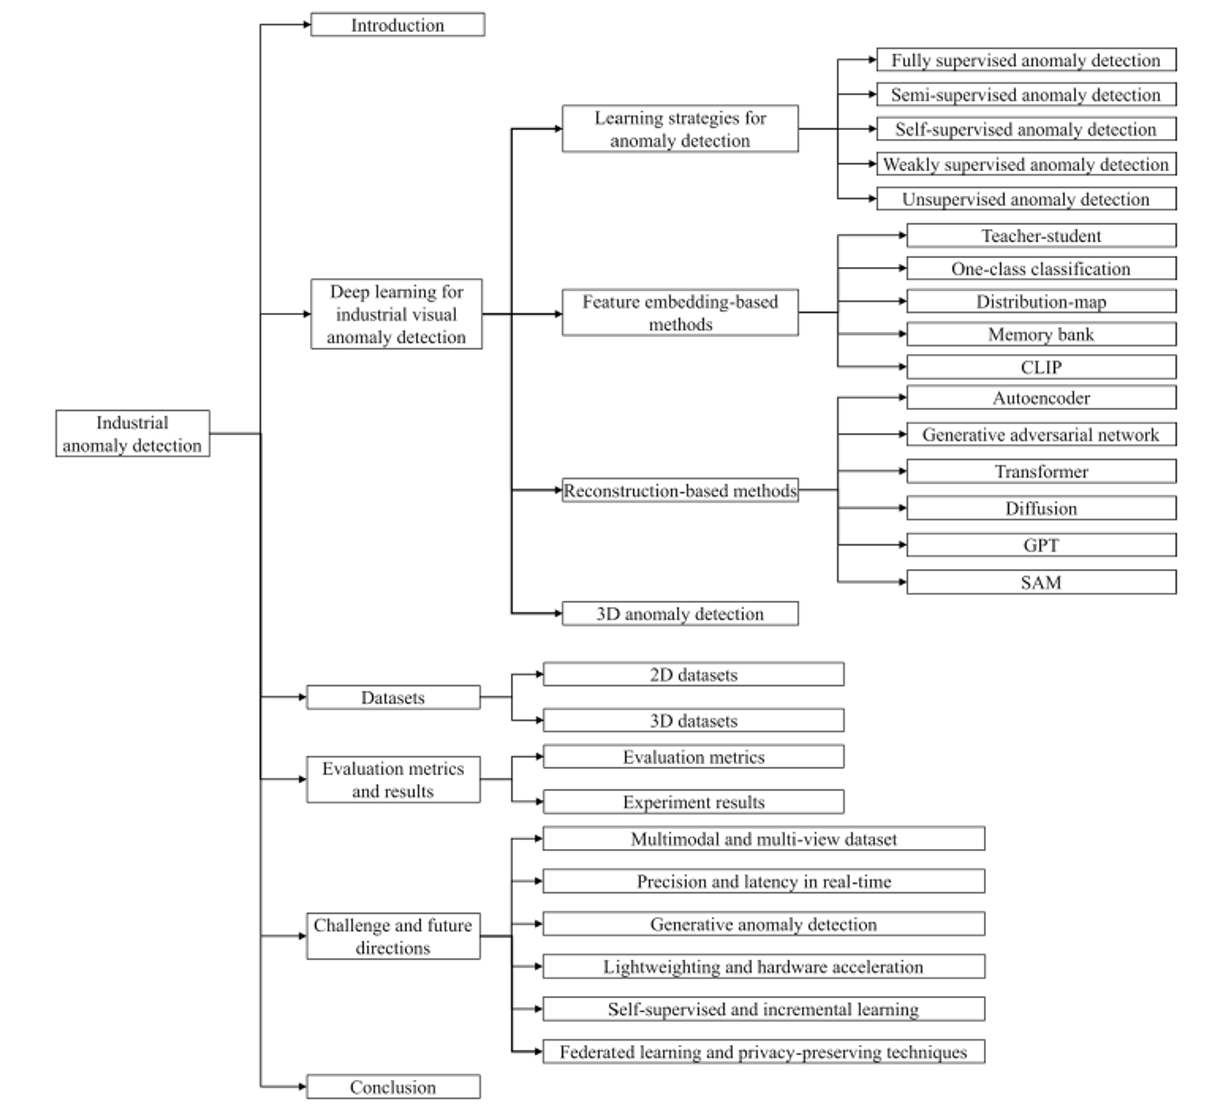
\includegraphics[width=0.9\linewidth]{images/Anomaly.png}
    \caption{Overview of the main methodological families in industrial visual anomaly detection.\cite{li_survey_2025}}
    \label{fig:ivad_taxonomy}
\end{figure}
